%======================================================================
\section{Numerical evaluation and tests on computed flows}\label{sec:numerics}
%======================================================================

\subsection{Wall functions and constants}
The wall functions \eqref{eq:Phi} were evaluated from the decomposition used in the proof. The half-space
kernels have closed forms in physical space; for example, for $d=2$,
\[
K^{\rm hs,ns}_{z,s}(y)=\frac1{8\pi}\ln\frac{b^2+y^2}{a^2+y^2}+\frac1{4\pi}\Big(\frac{a^2}{a^2+y^2}-\frac{b^2}{b^2+y^2}\Big)-\frac{zs}{2\pi}\frac{b^2-y^2}{(b^2+y^2)^2}.
\]
The slab corrections have smooth, exponentially decaying symbols. We transform them by FFT ($d=2$) or by Hankel
quadrature ($d=3$), after removing analytically the $|\kappa|$ cusp of the stress-free correction (which would
otherwise produce a slowly decaying $y^{-2}$ tail). For small $\kappa$ the symbols are evaluated in 50-digit
arithmetic. The slab Green's functions were checked against the exact sine series (stress-free; agreement to
$10^{-10}$) and against the collocation operator of the time-stepping code (no-slip; agreement to 10
significant figures).

Figure~\ref{fig:wall} confirms Lemma~\ref{lem:Phi}. A fit of $\Phi_{\rm ns}(z)/z^2-\frac12\nu_2\ln(1/z)$ on
$10^{-4}\le z\le10^{-2}$ gives the constant term $b=-0.430$ ($d=2$) and $-0.573$ ($d=3$); the slope agrees with
$\frac12\nu_2$ to three digits. For stress-free walls $\Phi_{\rm sf}(z)/z\to c_{\rm w}$. Evaluating the limit
directly, $c_{\rm w}=0.194366$ for $d=2$, both from the closed-form sine series and from the half-space and
correction split (agreement to $3\times10^{-8}$), and $c_{\rm w}=0.254086$ for $d=3$.

\paragraph{The slab-correction constants.} The suprema \eqref{eq:Cns} are taken over the compact rectangle
$Q=[0,\frac12]\times[0,1]$ of the parameters $(\zeta,s)$. We evaluated the norms on an $11\times21$ grid and
refined twice around the largest value, with grid spacing $0.003$ at the end. Each norm is computed as the
integral of the transformed kernel over $|y|\le40$ plus two analytic tails beyond that radius. The first is the
exact contribution of the stress-free cusp $-\frac s2\kappa e^{-\kappa}$. The second is the contribution of the
$|\kappa|^3$ term in the low-frequency expansion of Lemma~\ref{lem:corr}(i), whose kernel decays like
$|y|^{-4}$ ($n=1$) or $|y|^{-5}$ ($n=2$). The results are
\[
C_{\rm ns}\approx0.86155\ (d=2),\quad 1.17193\ (d=3);\qquad C_{\rm sf}\approx0.3183099\ (d=2),\quad 0.3849002\ (d=3).
\]
The no-slip maxima lie at $\zeta=0$ with $s=0.9125$ ($d=2$) and $s=0.90$ ($d=3$). The stress-free maxima lie at
the corner $(\zeta,s)=(0,1)$. There Lemma~\ref{lem:corr}(iii) gives the norm exactly as $\frac12\nu_1$, that is
$1/\pi=0.31830989$ and $2/(3\sqrt3)=0.38490018$, and the computed values agree with these to $1\times10^{-8}$
and $5\times10^{-8}$. The exact lower bound $C_{\rm sf}\ge\frac12\nu_1$ is a useful test: it catches any
truncation that loses part of the slowly decaying kernel tail.

Four further checks assess numerical sensitivity, without enclosing the remaining error. (i) Doubling the truncation radius to $80$ changes the norms at
the maximisers by at most $3\times10^{-6}$. (ii) For $n=1$ an independent evaluation, by adaptive quadrature in
$20$-digit arithmetic of the inverse cosine transform and of $|K|$ between its computed sign changes, agrees to
$2\times10^{-6}$. (iii) Between neighbouring grid points the no-slip values change by at most $2.5$ ($d=2$) and $3.5$ ($d=3$)
per unit change of $(\zeta,s)$, and the stress-free values by at most $0.45$; with the final spacing, this suggests that the true suprema exceed the grid maxima
by less than $0.007$ and $0.009$ (no-slip, $d=2$ and $3$) and $0.0011$ (stress-free). (iv) The Carlson majorants of
Lemma~\ref{lem:corr}(iii) involve only integrals of squares of the symbol and its derivatives, with no
oscillatory transform. Their sampled maxima are approximately $0.9703$ and $1.3031$ (no-slip) and
$0.4027$ and $0.5264$ (stress-free), for $d=2,3$. These are not continuum upper bounds:
inter-grid variation and quadrature remainders lack uniform enclosures. Finite-difference slopes and
truncation agreement do not supply them. The constants of
Theorem~\ref{thm:main} depend only weakly on these numbers. With the directly computed values,
$c_{\rm ns}=0.2046$ and $0.1871$ and $c_{\rm sf}=0.2698$ and $0.2454$; with the Carlson majorants,
$c_{\rm ns}=0.2036$ and $0.1863$ and $c_{\rm sf}=0.2535$ and $0.2255$. A further $10\%$ increase of $C_{\rm ns}$
or $C_{\rm sf}$ would lower $c_{\rm ns}$ by $0.4\%$ and $c_{\rm sf}$ by $2.4\%$. None of these computations is
interval-certified; Table~\ref{tab:status} records this.

\paragraph{The bound functional.} The explicit majorants of Lemma~\ref{lem:Phi} exceed the computed $\Phi$ on
$10^{-4}\le z\le\frac12$ by a factor of at least $2.8$ (no-slip) and $3.0$ (stress-free). As $z\to0$ the no-slip
factor tends to $2A/\nu_2=2.40$ ($d=2$) and $2.39$ ($d=3$). The functional $\mathfrak B[\Lambda\Phi]$ was
integrated on a graded grid. Table~\ref{tab:bound} gives representative values. Over $\Lambda\ge e^3$ the
quantity $\mathfrak B[\Lambda\Phi_{\rm ns}](\Lambda\ln\Lambda)^{1/3}$ lies between $1.46$ and $2.70$ for $d=2$
($1.31$--$2.39$ for $d=3$), decreasing slowly to the asymptotic value $1.41$ ($1.28$) of
Proposition~\ref{prop:sharp}. The estimated prefactor $c_{\rm ns}\approx0.205$ of Theorem~\ref{thm:main} is therefore
conservative by a factor of about $7$. For stress-free walls, $\mathfrak B\Lambda^{1/2}$ lies in $[1.81,2.56]$
($d=2$) and $[1.58,2.23]$ ($d=3$). These values use the computed wall functions, not the constants
$C_{\rm ns}$ and $C_{\rm sf}$. The wall functions are norms of full slab kernels, whose symbols are analytic and
even in $\kappa$; their kernels decay exponentially, so the truncation at $|y|=40$ is immaterial for them.

\begin{figure}[t]\centering
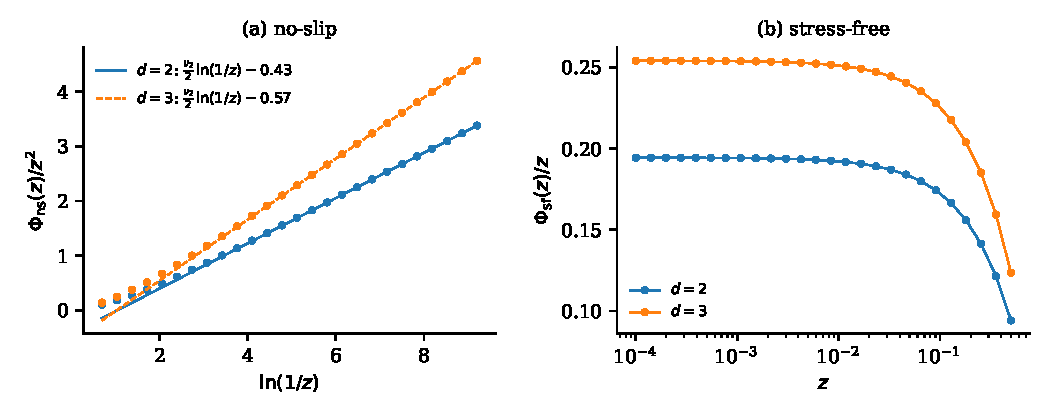
\includegraphics[width=\textwidth]{fig1_wall_functions.pdf}
\caption{Wall functions. (a) $\Phi_{\rm ns}(z)/z^2$ against $\ln(1/z)$ for $d=2,3$ (symbols), with the
asymptote $\frac12\nu_2\ln(1/z)+b$ of Lemma~\ref{lem:Phi} (lines). (b) $\Phi_{\rm sf}(z)/z$, which tends to
$c_{\rm w}$.}\label{fig:wall}
\end{figure}

\begin{table}[t]\centering
\caption{Uncertified numerical evaluation of $\mathfrak B[\Lambda\Phi_{\rm bc}]$ of Theorem~\ref{thm:main} ($\Lambda=\frac12R\mathcal T$).}\label{tab:bound}
\begin{tabular}{lcccc}\hline
$\Lambda$ & no-slip, $d=2$ & no-slip, $d=3$ & stress-free, $d=2$ & stress-free, $d=3$\\\hline
$10^{3}$ & $1.000\times10^{-1}$ & $8.700\times10^{-2}$ & $6.124\times10^{-2}$ & $5.305\times10^{-2}$ \\
$10^{4}$ & $3.739\times10^{-2}$ & $3.311\times10^{-2}$ & $1.846\times10^{-2}$ & $1.611\times10^{-2}$ \\
$10^{6}$ & $6.453\times10^{-3}$ & $5.774\times10^{-3}$ & $1.813\times10^{-3}$ & $1.586\times10^{-3}$ \\
$10^{8}$ & $1.221\times10^{-3}$ & $1.097\times10^{-3}$ & $1.810\times10^{-4}$ & $1.583\times10^{-4}$ \\
$10^{10}$ & $2.401\times10^{-4}$ & $2.160\times10^{-4}$ & $1.810\times10^{-5}$ & $1.583\times10^{-5}$ \\
$10^{12}$ & $4.818\times10^{-5}$ & $4.340\times10^{-5}$ & $1.811\times10^{-6}$ & $1.584\times10^{-6}$ \\
\hline\end{tabular}\end{table}


\subsection{Comparison with previous bounds and with simulations}
Figure~\ref{fig:bounds} compares the bound for $d=2$ with the bounds of \citet{ArslanRojas2025}, including their
explicit constants, and with simulated values of $F_B$. The exact expression underlying the solid curve is unconditional; its plotted numerical evaluation is not certified. It is
$\mathfrak B[\frac12R\mathcal T_{\max}\Phi]$ from Corollary~\ref{cor:R}, with $\mathcal T_{\max}=1.477$ for the
period-4 layer of the simulations. Two further curves show what \eqref{eq:mainbound} would give if the maximum
temperature were known not to exceed $1$ or the conductive value $\frac18$. They are conditional: neither ceiling
is proved, although every flow we computed stays below $\frac18$ over the windows we examined. At $R=10^9$ the
unconditional no-slip bound is $6.0\times10^{-4}$, against $1.9\times10^{-7}$ previously, and the stress-free
bound is $6.7\times10^{-5}$, against $5\times10^{-15}$. With $\mathcal T=\frac18$ these would rise to
$1.4\times10^{-3}$ and $2.3\times10^{-4}$. Over the simulated range $10^5\le R\le5\times10^9$, the no-slip fluxes
of \citet{ArslanRojas2025} exceed the unconditional bound by factors of $26$ to $500$. Our own simulations give
$\overline{F_B}=0.4435$ and $0.3620$ (no-slip) and $0.3916$ and $0.3200$ (stress-free) at $R=10^5$ and $10^6$:
$26$ to $150$ times the unconditional bound, and $10$ to $33$ times the bound evaluated with each window's measured
maximum temperature.

\begin{figure}[t]\centering
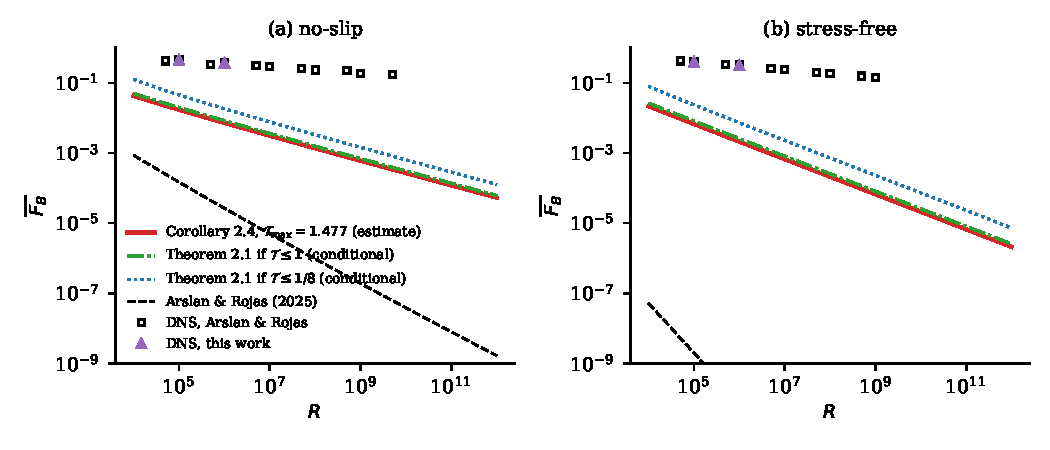
\includegraphics[width=\textwidth]{fig2_bounds.pdf}
\caption{Uncertified numerical evaluations of lower-bound formulas for $\overline{F_B}$, $d=2$. Solid red: Corollary~\ref{cor:R} with
$\mathcal T_{\max}\approx1.477$ (period 4). The formula, not its plotted decimals, is proved. Dash-dotted and dotted: \eqref{eq:mainbound} under the
unproved assumptions $\mathcal T\le1$ and $\mathcal T\le\frac18$. Dashed: \citet{ArslanRojas2025}. Squares: their
simulations; triangles: ours.}\label{fig:bounds}
\end{figure}

\subsection{Solvers and validation}
We integrate \eqref{eq:ihc} in two dimensions with $N_x$ Fourier modes ($3/2$-rule dealiasing) and $N_z+1$
Chebyshev--Lobatto points. For each wavenumber, the map $\hat T_\kappa\mapsto\hat w_\kappa$ is precomputed by an
influence-matrix method that uses only two well-conditioned Dirichlet Helmholtz solves. Time stepping is
SBDF2 at unchanged step size, restarting with SBDF1 whenever the adaptive CFL-limited step changes.
The four windows contain 21, 68, 11 and 2 step changes, respectively; realised second-order accuracy is not established. Steady states are found by Newton's method
for mirror-symmetric rolls, with the Jacobian assembled exactly by batched linearisation (checked against
finite differences to $6\times10^{-12}$). The codes reproduce:
\begin{itemize}
\item the linear thresholds $\mathrm{Ra}_c=1707.76$ at $k=3.116$ (Rayleigh--B\'enard, no-slip) and
$R_L=37\,325.2$ at $k=3.999$ (internally heated, no-slip) \citep{Goluskin2016};
\item the benchmark Nusselt numbers of \citet{Blankenbach1989}, $4.884409$, $10.534095$ and $21.972465$ at
$\mathrm{Ra}=10^4,10^5,10^6$ (free-slip square cell, which is half of our mirror-symmetric roll of period 2 between
stress-free plates), to relative errors $4\times10^{-8}$, $2\times10^{-8}$ and $2\times10^{-7}$;
\item agreement between time-stepping and Newton for a steady roll (Nu equal to $10^{-10}$);
\item the internally heated simulations of \citet{ArslanRojas2025} (no-slip, aspect ratio 4). At $R=10^5$ our
run settles on a steady state with $F_B=0.44291$, against their $0.4429$; at $R=10^6$ our time average is
$0.3620$, against their $0.367$.
\end{itemize}
In the simulations, the largest Fourier coefficient of $T$ in the last tenth of the retained modes is below
$10^{-8}$ of the largest coefficient in every stored snapshot, and the corresponding Chebyshev tail is below
$2\times10^{-8}$. Time averages are physical-time integrals: every diagnostic is evaluated at the same time level
as the state, and the trapezoidal rule is applied over every step of the adaptive integration. The averaged heat
balance $\frac d{dt}\langle T\rangle=1-F_B-F_T$ then holds over each window to within $10^{-8}$, which checks the
bookkeeping. Each run was continued from the state at the end of an earlier run, and averaged over a later
window, of length 4 ($R=10^5$) or 3 ($R=10^6$) diffusive times.

The flows are less turbulent than their Rayleigh numbers might suggest. At $R=10^5$, with either boundary
condition, and at $R=10^6$ with stress-free walls, the flow spends $76$--$89\%$ of the window at a steady state
($F_B=0.44291$, $0.39158$ and $0.32024$) and leaves it in one or two bursts, during which $F_B$ ranges over
$0.43$--$0.46$, $0.38$--$0.43$ and $0.31$--$0.36$ before returning. Only the no-slip flow at $R=10^6$ is
time-dependent throughout. For intermittent flows a window of this length samples only one or two bursts, so the
long-time mean, which depends on how often bursts recur, has no justified uncertainty estimate from these
eight sub-blocks. Their spread is descriptive only. These runs are finite-window illustrations, not temporally
or statistically converged estimates. Heat-budget closure checks bookkeeping, not temporal accuracy. Step,
longer-window and restart sensitivity would be needed before quantitative long-time claims; none are made here.

\subsection{Testing the proof on simulated flows}\label{sec:tests}
Table~\ref{tab:dns} reports, for each simulation, the time-averaged flux, the maximum temperature
$\mathcal T_\tau$ over the averaging window, and two ratios that the proof requires to be at most one. The first is
$\max_zJ/(W\Theta)$, where $W(z)=\max_{x,t}|w|$; this is the step $J\le m\Theta$ of Lemma~\ref{lem:IF}. The
second is $\max_zW/(\frac12R\mathcal T_\tau\Phi)$; this is Lemma~\ref{lem:rep} applied over the window. Both hold
at the sampled heights with wide margins, not as certified continuum enclosures. The last two columns apply Lemma~\ref{lem:IF} to the window itself: the window
mean of $F_B$ must be at least $\mathfrak B[\frac12R\mathcal T_\tau\Phi]-\mathcal T_\tau/\tau$, which is a weak
statement for windows this short (it is negative in two cases) but is satisfied by a wide margin. Two features
stand out.
\begin{enumerate}
\item The velocity bound is not attained. The measured $\max|w|$ reaches at most about a third of the kernel
bound, and only $11$--$20\%$ of it in the lower fifth of the layer. The kernel bound assumes a temperature
pattern of amplitude $\mathcal T$, matched to the kernel at every height; real temperature fields are far from
that.
\item The flux bound is far from attained (Figure~\ref{fig:profiles}). Over the lower third of the layer
the convective flux $J$ is below $1\%$ of its maximum, and in places slightly \emph{negative}: plumes penetrating
the stably stratified bottom layer carry a little heat downwards. The proof's extremal configuration needs
$J\approx z-F_B$ there, that is, the heat generated near the base carried upward at the maximal rate. Real flows
instead leave this region almost entirely to conduction. From \eqref{eq:balance}, if
$\int_0^zJ\le0$ for all $z\le h$ then $\overline{F_B}\ge h/2$; this is why $F_B$ decays so slowly in
simulations.
\end{enumerate}
The maximum temperature over the window decreases with $R$ ($\mathcal T_\tau=0.115$ and $0.079$ at $R=10^5$ and
$10^6$ for no-slip walls; $0.097$ and $0.069$ for stress-free walls). Over a finite window this is an observation,
not a bound on the long-time maximum $\mathcal T$.

\paragraph{The profile hypothesis of \citet{ChenEtAl2024}.}
Their Eq.~(14) assumes the statistically stationary profile inequality
$\Theta(z)\le\min\{F_Bz,(1-F_B)(1-z)\}$. All four full-window profiles pass the original interior-grid test,
with largest ratios $0.99946$--$0.99965$, but this does not establish the continuous inequality.
For no-slip $R=10^6$ the reconstructed finite-window means are
\[
F_B=0.3620304571851,\qquad F_T=0.6380454938113,
\qquad \frac{F_T}{1-F_B}=1.000119051132>1.
\]
Since $\Theta(1)=0$ and $-\Theta'(1)=F_T$, the last ratio is the limiting profile/triangle ratio at the top wall.
The continuous finite-window profile must therefore exceed the triangle near that wall. At $1-z=10^{-4}$
the spectral interpolant gives a ratio about $1.00004068$; the nearest interior grid point is farther away,
at $1-z\approx6.0227\times10^{-4}$. Checking derivative roots of the two polynomial differences on either side
of the triangle apex finds a maximal excess approximately $2.8843\times10^{-9}$ at $z\approx0.99992405$.
These are floating-point interpolant diagnostics, not validated enclosures of the PDE solution.

The effect is explained by finite-window cooling: $1-F_B-F_T=\Delta\langle T\rangle/\tau<0$.
It is not a counterexample to the stationary or infinite-time hypothesis. The revised checker reports grid tests,
boundary-slope compatibility and off-grid interpolant extrema separately; no grid pass is called a continuous proof.
Six of 32 sub-blocks already violate the sampled test. The remaining full-window interpolants have no violation
detected at the declared tolerance, which likewise does not prove the stationary hypothesis.
The theorem does not use that hypothesis.

\begin{table}[t]\centering\footnotesize
\caption{Simulations ($d=2$, period 4, $256\times64$ modes), averaged in physical time over the window
$[t_0,t_0+\tau]$ shown, and the descriptive range over eight sub-blocks (not a long-time confidence interval). The sixth column is the
window's heat imbalance, which equals $-\Delta\langle T\rangle/\tau$ exactly. $\mathcal T_\tau$ is the
maximum temperature over the window. The two ratios must not exceed one (Lemmas~\ref{lem:IF} and \ref{lem:rep}); $\min J$ is
over $z<0.2$. The last two columns are $\mathfrak B[\frac12R\mathcal T_\tau\Phi]$ and the finite-window value
$\mathfrak B[\frac12R\mathcal T_\tau\Phi]-\mathcal T_\tau/\tau$ whose exact formula occurs in Lemma~\ref{lem:IF}; these decimal evaluations are uncertified.}\label{tab:dns}
\setlength{\tabcolsep}{3pt}
\resizebox{\textwidth}{!}{%
\begin{tabular}{lccccccccccc}\hline
walls & $R$ & window & $\overline{F_B}$ & block means & $\overline{F_B}+\overline{F_T}-1$ & $\mathcal T_\tau$ & $\max\frac{J}{W\Theta}$ & $\max\frac{W}{\frac12R\mathcal T_\tau\Phi}$ & $\min J$ & $\mathfrak B$ & $\mathfrak B-\frac{\mathcal T_\tau}{\tau}$\\\hline
no-slip & $10^{5}$ & $[3,7]$ & 0.4435 & 0.4429--0.4474 & $-7.7\times10^{-9}$ & 0.1149 & 0.090 & 0.314 & $-$0.0029 & 0.0468 & 0.0181 \\
no-slip & $10^{6}$ & $[2,5]$ & 0.3620 & 0.3609--0.3629 & $7.6\times10^{-5}$ & 0.0790 & 0.055 & 0.339 & $-$0.0077 & 0.0218 & $-$0.0046 \\
stress-free & $10^{5}$ & $[3,7]$ & 0.3916 & 0.3910--0.3927 & $-2.3\times10^{-12}$ & 0.0974 & 0.074 & 0.359 & $-$0.0329 & 0.0267 & 0.0024 \\
stress-free & $10^{6}$ & $[2,5]$ & 0.3200 & 0.3192--0.3203 & $-1.6\times10^{-6}$ & 0.0694 & 0.043 & 0.251 & $-$0.0307 & 0.0098 & $-$0.0133 \\
\hline\end{tabular}}\end{table}


\begin{figure}[t]\centering
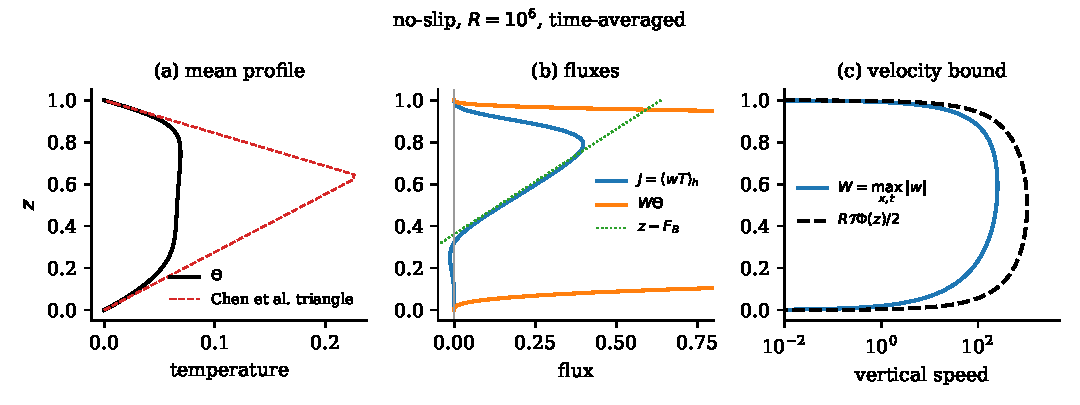
\includegraphics[width=\textwidth]{fig3_ih_ns_R1e+06_G4_256x64_cont.pdf}
\caption{Simulated no-slip flow at $R=10^6$ (finite-window averages, not converged statistics). (a) Mean temperature and the triangle of the
\citet{ChenEtAl2024} hypothesis; the near-wall violation is too small to resolve at this scale. (b) Convective flux $J$, the bound $W\Theta$ used in Lemma~\ref{lem:IF}, and
the profile $z-F_B$ that the extremal configuration would need. (c) Measured maximal vertical speed against
the kernel bound of Lemma~\ref{lem:rep}.}\label{fig:profiles}
\end{figure}
